\begin{figure}[H]
\centering
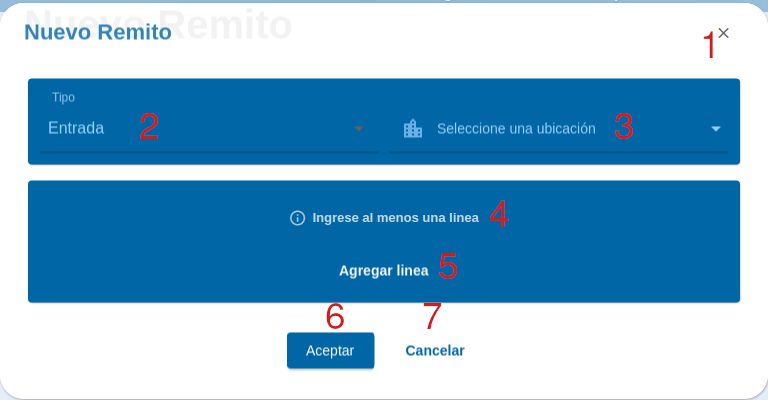
\includegraphics[width=\textwidth,height=\textheight,keepaspectratio]{Escenarios/AD-17-00}
\caption{Escenario - AD-17-00}
\label{fig:AD-17-00}
\end{figure}
Este es el escenario que permite a los usuarios crear remitos. Con el botón \textbf{AD-17-01} se podrá cerrar la ventana y volver al escenario \textbf{AD-16-00}.
El campo \textbf{AD-17-02} permite al usuario indicar tipo de remito que está por crear.  La lista desplegable \textbf{AD-17-03} aparecerá en caso que se trate de un remito de entrada, y le permitirá al usuario indicar en que ubicación se están recibiendo los productos.
El campo \textbf{AD-17-04} se muestra cuando la venta no tiene asociado ninguna linea de remito. El boton \textbf{AD-17-05} permite al usuario crear una linea de remito y asociarla al remito, navega al escenario \textbf{AD-18-00}. Si el usuario hace click en el botón \textbf{AD-17-06} creará el remito y navegará al escenario \textbf{AD-16-00}, si hace click en el botón \textbf{AD-17-07} cerrará la ventana navegando al escenario \textbf{AD-16-00}.
\\
